


% Header, overrides base

    % Make sure that the sphinx doc style knows who it inherits from.
    \def\sphinxdocclass{article}

    % Declare the document class
    \documentclass[letterpaper,10pt,english]{/usr/share/sphinx/texinputs/sphinxhowto}

    % Imports
    \usepackage[utf8]{inputenc}
    \DeclareUnicodeCharacter{00A0}{\\nobreakspace}
    \usepackage[T1]{fontenc}
    \usepackage{babel}
    \usepackage{times}
    \usepackage{import}
    \usepackage[Bjarne]{/usr/share/sphinx/texinputs/fncychap}
    \usepackage{longtable}
    \usepackage{/usr/share/sphinx/texinputs/sphinx}
    \usepackage{multirow}

    \usepackage{amsmath}
    \usepackage{amssymb}
    \usepackage{ucs}
    \usepackage{enumerate}

    % Used to make the Input/Output rules follow around the contents.
    \usepackage{needspace}

    % Pygments requirements
    \usepackage{fancyvrb}
    \usepackage{color}
    % ansi colors additions
    \definecolor{darkgreen}{rgb}{.12,.54,.11}
    \definecolor{lightgray}{gray}{.95}
    \definecolor{brown}{rgb}{0.54,0.27,0.07}
    \definecolor{purple}{rgb}{0.5,0.0,0.5}
    \definecolor{darkgray}{gray}{0.25}
    \definecolor{lightred}{rgb}{1.0,0.39,0.28}
    \definecolor{lightgreen}{rgb}{0.48,0.99,0.0}
    \definecolor{lightblue}{rgb}{0.53,0.81,0.92}
    \definecolor{lightpurple}{rgb}{0.87,0.63,0.87}
    \definecolor{lightcyan}{rgb}{0.5,1.0,0.83}

    % Needed to box output/input
    \usepackage{tikz}
        \usetikzlibrary{calc,arrows,shadows}
    \usepackage[framemethod=tikz]{mdframed}

    \usepackage{alltt}

    % Used to load and display graphics
    \usepackage{graphicx}
    \graphicspath{ {figs/} }
    \usepackage[Export]{adjustbox} % To resize

    % used so that images for notebooks which have spaces in the name can still be included
    \usepackage{grffile}


    % For formatting output while also word wrapping.
    \usepackage{listings}
    \lstset{breaklines=true}
    \lstset{basicstyle=\small\ttfamily}
    \def\smaller{\fontsize{9.5pt}{9.5pt}\selectfont}

    %Pygments definitions
    
\makeatletter
\def\PY@reset{\let\PY@it=\relax \let\PY@bf=\relax%
    \let\PY@ul=\relax \let\PY@tc=\relax%
    \let\PY@bc=\relax \let\PY@ff=\relax}
\def\PY@tok#1{\csname PY@tok@#1\endcsname}
\def\PY@toks#1+{\ifx\relax#1\empty\else%
    \PY@tok{#1}\expandafter\PY@toks\fi}
\def\PY@do#1{\PY@bc{\PY@tc{\PY@ul{%
    \PY@it{\PY@bf{\PY@ff{#1}}}}}}}
\def\PY#1#2{\PY@reset\PY@toks#1+\relax+\PY@do{#2}}

\expandafter\def\csname PY@tok@gd\endcsname{\def\PY@tc##1{\textcolor[rgb]{0.63,0.00,0.00}{##1}}}
\expandafter\def\csname PY@tok@gu\endcsname{\let\PY@bf=\textbf\def\PY@tc##1{\textcolor[rgb]{0.50,0.00,0.50}{##1}}}
\expandafter\def\csname PY@tok@gt\endcsname{\def\PY@tc##1{\textcolor[rgb]{0.00,0.27,0.87}{##1}}}
\expandafter\def\csname PY@tok@gs\endcsname{\let\PY@bf=\textbf}
\expandafter\def\csname PY@tok@gr\endcsname{\def\PY@tc##1{\textcolor[rgb]{1.00,0.00,0.00}{##1}}}
\expandafter\def\csname PY@tok@cm\endcsname{\let\PY@it=\textit\def\PY@tc##1{\textcolor[rgb]{0.25,0.50,0.50}{##1}}}
\expandafter\def\csname PY@tok@vg\endcsname{\def\PY@tc##1{\textcolor[rgb]{0.10,0.09,0.49}{##1}}}
\expandafter\def\csname PY@tok@m\endcsname{\def\PY@tc##1{\textcolor[rgb]{0.40,0.40,0.40}{##1}}}
\expandafter\def\csname PY@tok@mh\endcsname{\def\PY@tc##1{\textcolor[rgb]{0.40,0.40,0.40}{##1}}}
\expandafter\def\csname PY@tok@go\endcsname{\def\PY@tc##1{\textcolor[rgb]{0.53,0.53,0.53}{##1}}}
\expandafter\def\csname PY@tok@ge\endcsname{\let\PY@it=\textit}
\expandafter\def\csname PY@tok@vc\endcsname{\def\PY@tc##1{\textcolor[rgb]{0.10,0.09,0.49}{##1}}}
\expandafter\def\csname PY@tok@il\endcsname{\def\PY@tc##1{\textcolor[rgb]{0.40,0.40,0.40}{##1}}}
\expandafter\def\csname PY@tok@cs\endcsname{\let\PY@it=\textit\def\PY@tc##1{\textcolor[rgb]{0.25,0.50,0.50}{##1}}}
\expandafter\def\csname PY@tok@cp\endcsname{\def\PY@tc##1{\textcolor[rgb]{0.74,0.48,0.00}{##1}}}
\expandafter\def\csname PY@tok@gi\endcsname{\def\PY@tc##1{\textcolor[rgb]{0.00,0.63,0.00}{##1}}}
\expandafter\def\csname PY@tok@gh\endcsname{\let\PY@bf=\textbf\def\PY@tc##1{\textcolor[rgb]{0.00,0.00,0.50}{##1}}}
\expandafter\def\csname PY@tok@ni\endcsname{\let\PY@bf=\textbf\def\PY@tc##1{\textcolor[rgb]{0.60,0.60,0.60}{##1}}}
\expandafter\def\csname PY@tok@nl\endcsname{\def\PY@tc##1{\textcolor[rgb]{0.63,0.63,0.00}{##1}}}
\expandafter\def\csname PY@tok@nn\endcsname{\let\PY@bf=\textbf\def\PY@tc##1{\textcolor[rgb]{0.00,0.00,1.00}{##1}}}
\expandafter\def\csname PY@tok@no\endcsname{\def\PY@tc##1{\textcolor[rgb]{0.53,0.00,0.00}{##1}}}
\expandafter\def\csname PY@tok@na\endcsname{\def\PY@tc##1{\textcolor[rgb]{0.49,0.56,0.16}{##1}}}
\expandafter\def\csname PY@tok@nb\endcsname{\def\PY@tc##1{\textcolor[rgb]{0.00,0.50,0.00}{##1}}}
\expandafter\def\csname PY@tok@nc\endcsname{\let\PY@bf=\textbf\def\PY@tc##1{\textcolor[rgb]{0.00,0.00,1.00}{##1}}}
\expandafter\def\csname PY@tok@nd\endcsname{\def\PY@tc##1{\textcolor[rgb]{0.67,0.13,1.00}{##1}}}
\expandafter\def\csname PY@tok@ne\endcsname{\let\PY@bf=\textbf\def\PY@tc##1{\textcolor[rgb]{0.82,0.25,0.23}{##1}}}
\expandafter\def\csname PY@tok@nf\endcsname{\def\PY@tc##1{\textcolor[rgb]{0.00,0.00,1.00}{##1}}}
\expandafter\def\csname PY@tok@si\endcsname{\let\PY@bf=\textbf\def\PY@tc##1{\textcolor[rgb]{0.73,0.40,0.53}{##1}}}
\expandafter\def\csname PY@tok@s2\endcsname{\def\PY@tc##1{\textcolor[rgb]{0.73,0.13,0.13}{##1}}}
\expandafter\def\csname PY@tok@vi\endcsname{\def\PY@tc##1{\textcolor[rgb]{0.10,0.09,0.49}{##1}}}
\expandafter\def\csname PY@tok@nt\endcsname{\let\PY@bf=\textbf\def\PY@tc##1{\textcolor[rgb]{0.00,0.50,0.00}{##1}}}
\expandafter\def\csname PY@tok@nv\endcsname{\def\PY@tc##1{\textcolor[rgb]{0.10,0.09,0.49}{##1}}}
\expandafter\def\csname PY@tok@s1\endcsname{\def\PY@tc##1{\textcolor[rgb]{0.73,0.13,0.13}{##1}}}
\expandafter\def\csname PY@tok@sh\endcsname{\def\PY@tc##1{\textcolor[rgb]{0.73,0.13,0.13}{##1}}}
\expandafter\def\csname PY@tok@sc\endcsname{\def\PY@tc##1{\textcolor[rgb]{0.73,0.13,0.13}{##1}}}
\expandafter\def\csname PY@tok@sx\endcsname{\def\PY@tc##1{\textcolor[rgb]{0.00,0.50,0.00}{##1}}}
\expandafter\def\csname PY@tok@bp\endcsname{\def\PY@tc##1{\textcolor[rgb]{0.00,0.50,0.00}{##1}}}
\expandafter\def\csname PY@tok@c1\endcsname{\let\PY@it=\textit\def\PY@tc##1{\textcolor[rgb]{0.25,0.50,0.50}{##1}}}
\expandafter\def\csname PY@tok@kc\endcsname{\let\PY@bf=\textbf\def\PY@tc##1{\textcolor[rgb]{0.00,0.50,0.00}{##1}}}
\expandafter\def\csname PY@tok@c\endcsname{\let\PY@it=\textit\def\PY@tc##1{\textcolor[rgb]{0.25,0.50,0.50}{##1}}}
\expandafter\def\csname PY@tok@mf\endcsname{\def\PY@tc##1{\textcolor[rgb]{0.40,0.40,0.40}{##1}}}
\expandafter\def\csname PY@tok@err\endcsname{\def\PY@bc##1{\setlength{\fboxsep}{0pt}\fcolorbox[rgb]{1.00,0.00,0.00}{1,1,1}{\strut ##1}}}
\expandafter\def\csname PY@tok@kd\endcsname{\let\PY@bf=\textbf\def\PY@tc##1{\textcolor[rgb]{0.00,0.50,0.00}{##1}}}
\expandafter\def\csname PY@tok@ss\endcsname{\def\PY@tc##1{\textcolor[rgb]{0.10,0.09,0.49}{##1}}}
\expandafter\def\csname PY@tok@sr\endcsname{\def\PY@tc##1{\textcolor[rgb]{0.73,0.40,0.53}{##1}}}
\expandafter\def\csname PY@tok@mo\endcsname{\def\PY@tc##1{\textcolor[rgb]{0.40,0.40,0.40}{##1}}}
\expandafter\def\csname PY@tok@kn\endcsname{\let\PY@bf=\textbf\def\PY@tc##1{\textcolor[rgb]{0.00,0.50,0.00}{##1}}}
\expandafter\def\csname PY@tok@mi\endcsname{\def\PY@tc##1{\textcolor[rgb]{0.40,0.40,0.40}{##1}}}
\expandafter\def\csname PY@tok@gp\endcsname{\let\PY@bf=\textbf\def\PY@tc##1{\textcolor[rgb]{0.00,0.00,0.50}{##1}}}
\expandafter\def\csname PY@tok@o\endcsname{\def\PY@tc##1{\textcolor[rgb]{0.40,0.40,0.40}{##1}}}
\expandafter\def\csname PY@tok@kr\endcsname{\let\PY@bf=\textbf\def\PY@tc##1{\textcolor[rgb]{0.00,0.50,0.00}{##1}}}
\expandafter\def\csname PY@tok@s\endcsname{\def\PY@tc##1{\textcolor[rgb]{0.73,0.13,0.13}{##1}}}
\expandafter\def\csname PY@tok@kp\endcsname{\def\PY@tc##1{\textcolor[rgb]{0.00,0.50,0.00}{##1}}}
\expandafter\def\csname PY@tok@w\endcsname{\def\PY@tc##1{\textcolor[rgb]{0.73,0.73,0.73}{##1}}}
\expandafter\def\csname PY@tok@kt\endcsname{\def\PY@tc##1{\textcolor[rgb]{0.69,0.00,0.25}{##1}}}
\expandafter\def\csname PY@tok@ow\endcsname{\let\PY@bf=\textbf\def\PY@tc##1{\textcolor[rgb]{0.67,0.13,1.00}{##1}}}
\expandafter\def\csname PY@tok@sb\endcsname{\def\PY@tc##1{\textcolor[rgb]{0.73,0.13,0.13}{##1}}}
\expandafter\def\csname PY@tok@k\endcsname{\let\PY@bf=\textbf\def\PY@tc##1{\textcolor[rgb]{0.00,0.50,0.00}{##1}}}
\expandafter\def\csname PY@tok@se\endcsname{\let\PY@bf=\textbf\def\PY@tc##1{\textcolor[rgb]{0.73,0.40,0.13}{##1}}}
\expandafter\def\csname PY@tok@sd\endcsname{\let\PY@it=\textit\def\PY@tc##1{\textcolor[rgb]{0.73,0.13,0.13}{##1}}}

\def\PYZbs{\char`\\}
\def\PYZus{\char`\_}
\def\PYZob{\char`\{}
\def\PYZcb{\char`\}}
\def\PYZca{\char`\^}
\def\PYZam{\char`\&}
\def\PYZlt{\char`\<}
\def\PYZgt{\char`\>}
\def\PYZsh{\char`\#}
\def\PYZpc{\char`\%}
\def\PYZdl{\char`\$}
\def\PYZhy{\char`\-}
\def\PYZsq{\char`\'}
\def\PYZdq{\char`\"}
\def\PYZti{\char`\~}
% for compatibility with earlier versions
\def\PYZat{@}
\def\PYZlb{[}
\def\PYZrb{]}
\makeatother


    %Set pygments styles if needed...
    
        \definecolor{nbframe-border}{rgb}{0.867,0.867,0.867}
        \definecolor{nbframe-bg}{rgb}{0.969,0.969,0.969}
        \definecolor{nbframe-in-prompt}{rgb}{0.0,0.0,0.502}
        \definecolor{nbframe-out-prompt}{rgb}{0.545,0.0,0.0}

        \newenvironment{ColorVerbatim}
        {\begin{mdframed}[%
            roundcorner=1.0pt, %
            backgroundcolor=nbframe-bg, %
            userdefinedwidth=1\linewidth, %
            leftmargin=0.1\linewidth, %
            innerleftmargin=0pt, %
            innerrightmargin=0pt, %
            linecolor=nbframe-border, %
            linewidth=1pt, %
            usetwoside=false, %
            everyline=true, %
            innerlinewidth=3pt, %
            innerlinecolor=nbframe-bg, %
            middlelinewidth=1pt, %
            middlelinecolor=nbframe-bg, %
            outerlinewidth=0.5pt, %
            outerlinecolor=nbframe-border, %
            needspace=0pt
        ]}
        {\end{mdframed}}
        
        \newenvironment{InvisibleVerbatim}
        {\begin{mdframed}[leftmargin=0.1\linewidth,innerleftmargin=3pt,innerrightmargin=3pt, userdefinedwidth=1\linewidth, linewidth=0pt, linecolor=white, usetwoside=false]}
        {\end{mdframed}}

        \renewenvironment{Verbatim}[1][\unskip]
        {\begin{alltt}\smaller}
        {\end{alltt}}
    

    % Help prevent overflowing lines due to urls and other hard-to-break 
    % entities.  This doesn't catch everything...
    \sloppy

    % Document level variables
    \title{Adriaan Riet Exam\_1 Problem 2}
    \date{February 20, 2015}
    \release{}
    \author{Unknown Author}
    \renewcommand{\releasename}{}

    % TODO: Add option for the user to specify a logo for his/her export.
    \newcommand{\sphinxlogo}{}

    % Make the index page of the document.
    \makeindex

    % Import sphinx document type specifics.
     


% Body

    % Start of the document
    \begin{document}

        
            \maketitle
        

        


        
        \part{ChEn 541: Exam 1: Winter 2015}\part{Due Friday October 20, BEFORE 9:00 AM}\part{Problem 2}\section{Open book, open notes. Closed homework, homework solutions, and closed
code examples. You may use the internet for Matlab and Python help only.}\subsection{Part a}A chemical reaction occurs in a continuous stirred tank reactor (CSTR).
There is an inlet, and an outlet. The contents are perfectly mixed and
the outlet composition is the same as the reactor composition.

The reactions are

A + B --\textgreater{} C (reaction 1)

B + C --\textgreater{} D (reaction 2)

The reaction rates for the species are given by \[\begin{align} 
r_A &= -k_1[A][B] \\
r_B &= -k_1[A][B] - k_2[B][C] \\
r_C &= k_1[A][B] - k_2[B][C] \\
r_D &= k_2[B][C]
\end{align}\]

The mass balance for each species in the CSTR is
\[ \frac{d[Y]}{dt} = \frac{[Y]_{in}-[Y]}{\tau} + r,\] where $[Y]$ is one
of $[A]$, $[B]$, $[C]$, or $[D]$. Also, $\tau$ is the residence time in
the reactor (volume divided by volumetric flow rate).Solve for the concentrations $[Y]$ as functions of time to an end time
of $5\tau$ as described below. Also solve for the selectivity
$S=C/(C+D)$, where C is a desired product and D is undesired. (This is
initially undefined, so set the initial selectivity to 1.0.

The initial concentration in the tank is $[B]_0 = 1.0$ and all other
species are zero.

The inlet concentrations are $[A]_{in} = 1.0$, and $[B]_{in} = 1.0$.

Take $\tau=10.0$, $k_1=1.0$, $k_2=5.0$. Use an initial stepsize of
$dt=0.01$.

You should plot the concentrations and selectivity on the same plot.
(Include a legend.) Use a linestyle that includes symbols so the step
size is clear. On a separate plot, show the stepsize versus time. Use a
log scale for the stepsize.

You should solve the problem using the Implicit Euler method. This is a
nonlinear, multidimensional problem. You will need a nonlinear solver.
Use Newton's method with an analytic Jacobian. You can use a built-in
(Matlab or Python) linear solver. Set the step size using the step
doubling technique. Use a relative tolerance of 0.005 for all error
testing, and use the 2-norm. You may want to solve this in steps, making
sure things work before adding complexity.In order to solve this problem, we need a general formula for implicit
Euler.

$\vec{y}_{n+1} = \vec{y}_n + h\left[\vec{f}(\vec{y}_{n+1})\right]$

Use Newton's method
identity.$\vec{y}_{n+1} \approx \vec{y}_n + h\left[\vec{f}(\vec{y}_n) + \frac{d\vec{f}}{d\vec{y}}\Big\vert_{\vec{y}_n}\cdot (\vec{y}_{n+1} - \vec{y}_n)\right]$

$\vec{y}_{n+1} - \vec{y}_n\approx h\left[\vec{f}(\vec{y}_n) + \frac{d\vec{f}}{d\vec{y}}\Big\vert_{\vec{y}_n}\cdot (\vec{y}_{n+1} - \vec{y}_n)\right]$

$\vec{y}_{n+1} - \vec{y}_n\approx h\vec{f}(\vec{y}_n) + h\frac{d\vec{f}}{d\vec{y}}\Big\vert_{\vec{y}_n}\cdot (\vec{y}_{n+1} - \vec{y}_n)$

$\left(\vec{y}_{n+1} - \vec{y}_n\right) -h\frac{d\vec{f}}{d\vec{y}}\Big\vert_{\vec{y}_n}\cdot (\vec{y}_{n+1} - \vec{y}_n) \approx h\vec{f}(\vec{y}_n)$

$\left(\mathbf{I} -h\frac{d\vec{f}}{d\vec{y}}\Big\vert_{\vec{y}_n}\right)\left(\vec{y}_{n+1} - \vec{y}_n\right) \approx h\vec{f}(\vec{y}_n)$

$\:\:\:\:\:\:\:\:\:\:\:\:\:\:\mathbf{A}\:\:\:\:\:\:\:\:\:\:\:\:\:\:\:\:\:\:\:\:\:\vec{x} \:\:\:\:\:\:\:\: \:\: =\:\:\:\:\:\:\:\:\:\vec{b}$

Solve $\mathbf{A}\vec{x}=\vec{b}$ with built in solver.

$\vec{y}_{n+1} = \vec{x}+\vec{y}_{n}$. $QED$

    % Make sure that atleast 4 lines are below the HR
    \needspace{4\baselineskip}

    
        \vspace{6pt}
        \makebox[0.1\linewidth]{\smaller\hfill\tt\color{nbframe-in-prompt}In\hspace{4pt}{[}1{]}:\hspace{4pt}}\\*
        \vspace{-2.65\baselineskip}
        \begin{ColorVerbatim}
            \vspace{-0.7\baselineskip}
            \begin{Verbatim}[commandchars=\\\{\}]
\PY{k+kn}{from} \PY{n+nn}{scipy.integrate} \PY{k+kn}{import} \PY{n}{odeint}
\PY{o}{\PYZpc{}}\PY{k}{matplotlib} \PY{n}{inline}
\PY{n}{myBool} \PY{o}{=} \PY{n+nb+bp}{False}
\end{Verbatim}

            
                \vspace{-0.2\baselineskip}
            
        \end{ColorVerbatim}
    


    % Make sure that atleast 4 lines are below the HR
    \needspace{4\baselineskip}

    
        \vspace{6pt}
        \makebox[0.1\linewidth]{\smaller\hfill\tt\color{nbframe-in-prompt}In\hspace{4pt}{[}2{]}:\hspace{4pt}}\\*
        \vspace{-2.65\baselineskip}
        \begin{ColorVerbatim}
            \vspace{-0.7\baselineskip}
            \begin{Verbatim}[commandchars=\\\{\}]
\PY{n}{tau} \PY{o}{=} \PY{l+m+mf}{10.}
\PY{n}{k1} \PY{o}{=} \PY{l+m+mf}{1.0}
\PY{n}{k2} \PY{o}{=} \PY{l+m+mf}{5.0}
\PY{n}{dt} \PY{o}{=} \PY{o}{.}\PY{l+m+mo}{01}
\PY{k}{def} \PY{n+nf}{f}\PY{p}{(}\PY{n}{y}\PY{p}{,}\PY{n}{t}\PY{o}{=}\PY{l+m+mi}{0}\PY{p}{)}\PY{p}{:}
    \PY{l+s+sd}{\PYZdq{}\PYZdq{}\PYZdq{}System of ODEs\PYZdq{}\PYZdq{}\PYZdq{}}
    \PY{n}{dy} \PY{o}{=} \PY{n}{np}\PY{o}{.}\PY{n}{zeros}\PY{p}{(}\PY{l+m+mi}{4}\PY{p}{)}
    \PY{c}{\PYZsh{}This is where we calculate the function}
    \PY{n}{dy}\PY{p}{[}\PY{l+m+mi}{0}\PY{p}{]} \PY{o}{=} \PY{p}{(}\PY{l+m+mi}{1}\PY{o}{\PYZhy{}}\PY{n}{y}\PY{p}{[}\PY{l+m+mi}{0}\PY{p}{]}\PY{p}{)}\PY{o}{/}\PY{n}{tau} \PY{o}{\PYZhy{}} \PY{n}{k1}\PY{o}{*}\PY{n}{y}\PY{p}{[}\PY{l+m+mi}{0}\PY{p}{]}\PY{o}{*}\PY{n}{y}\PY{p}{[}\PY{l+m+mi}{1}\PY{p}{]}
    \PY{n}{dy}\PY{p}{[}\PY{l+m+mi}{1}\PY{p}{]} \PY{o}{=} \PY{p}{(}\PY{l+m+mi}{1}\PY{o}{\PYZhy{}}\PY{n}{y}\PY{p}{[}\PY{l+m+mi}{1}\PY{p}{]}\PY{p}{)}\PY{o}{/}\PY{n}{tau} \PY{o}{\PYZhy{}} \PY{n}{k1}\PY{o}{*}\PY{n}{y}\PY{p}{[}\PY{l+m+mi}{0}\PY{p}{]}\PY{o}{*}\PY{n}{y}\PY{p}{[}\PY{l+m+mi}{1}\PY{p}{]} \PY{o}{\PYZhy{}} \PY{n}{k2}\PY{o}{*}\PY{n}{y}\PY{p}{[}\PY{l+m+mi}{1}\PY{p}{]}\PY{o}{*}\PY{n}{y}\PY{p}{[}\PY{l+m+mi}{2}\PY{p}{]}
    \PY{n}{dy}\PY{p}{[}\PY{l+m+mi}{2}\PY{p}{]} \PY{o}{=} \PY{o}{\PYZhy{}}\PY{n}{y}\PY{p}{[}\PY{l+m+mi}{2}\PY{p}{]}\PY{o}{/}\PY{n}{tau}    \PY{o}{+} \PY{n}{k1}\PY{o}{*}\PY{n}{y}\PY{p}{[}\PY{l+m+mi}{0}\PY{p}{]}\PY{o}{*}\PY{n}{y}\PY{p}{[}\PY{l+m+mi}{1}\PY{p}{]} \PY{o}{\PYZhy{}} \PY{n}{k2}\PY{o}{*}\PY{n}{y}\PY{p}{[}\PY{l+m+mi}{1}\PY{p}{]}\PY{o}{*}\PY{n}{y}\PY{p}{[}\PY{l+m+mi}{2}\PY{p}{]}
    \PY{n}{dy}\PY{p}{[}\PY{l+m+mi}{3}\PY{p}{]} \PY{o}{=} \PY{o}{\PYZhy{}}\PY{n}{y}\PY{p}{[}\PY{l+m+mi}{3}\PY{p}{]}\PY{o}{/}\PY{n}{tau}                   \PY{o}{+} \PY{n}{k2}\PY{o}{*}\PY{n}{y}\PY{p}{[}\PY{l+m+mi}{1}\PY{p}{]}\PY{o}{*}\PY{n}{y}\PY{p}{[}\PY{l+m+mi}{2}\PY{p}{]}
    \PY{k}{return} \PY{n}{dy}

\PY{k}{def} \PY{n+nf}{Jac}\PY{p}{(}\PY{n}{y}\PY{p}{)}\PY{p}{:}
    \PY{l+s+sd}{\PYZdq{}\PYZdq{}\PYZdq{}Analytical Jacobian to solve problem statement\PYZdq{}\PYZdq{}\PYZdq{}}
    \PY{n}{J} \PY{o}{=} \PY{n}{np}\PY{o}{.}\PY{n}{zeros}\PY{p}{(}\PY{p}{[}\PY{l+m+mi}{4}\PY{p}{,}\PY{l+m+mi}{4}\PY{p}{]}\PY{p}{)}
    \PY{n}{J}\PY{p}{[}\PY{l+m+mi}{0}\PY{p}{,}\PY{l+m+mi}{0}\PY{p}{]} \PY{o}{=} \PY{o}{\PYZhy{}}\PY{l+m+mi}{1}\PY{o}{/}\PY{n}{tau} \PY{o}{\PYZhy{}} \PY{n}{k1}\PY{o}{*}\PY{n}{y}\PY{p}{[}\PY{l+m+mi}{1}\PY{p}{]}
    \PY{n}{J}\PY{p}{[}\PY{l+m+mi}{0}\PY{p}{,}\PY{l+m+mi}{1}\PY{p}{]} \PY{o}{=}        \PY{o}{\PYZhy{}} \PY{n}{k1}\PY{o}{*}\PY{n}{y}\PY{p}{[}\PY{l+m+mi}{1}\PY{p}{]}
    \PY{n}{J}\PY{p}{[}\PY{l+m+mi}{0}\PY{p}{,}\PY{l+m+mi}{2}\PY{p}{]} \PY{o}{=}          \PY{n}{k1}\PY{o}{*}\PY{n}{y}\PY{p}{[}\PY{l+m+mi}{1}\PY{p}{]}
    \PY{n}{J}\PY{p}{[}\PY{l+m+mi}{0}\PY{p}{,}\PY{l+m+mi}{3}\PY{p}{]} \PY{o}{=} \PY{l+m+mi}{0}
    \PY{n}{J}\PY{p}{[}\PY{l+m+mi}{1}\PY{p}{,}\PY{l+m+mi}{0}\PY{p}{]} \PY{o}{=}        \PY{o}{\PYZhy{}} \PY{n}{k1}\PY{o}{*}\PY{n}{y}\PY{p}{[}\PY{l+m+mi}{0}\PY{p}{]}
    \PY{n}{J}\PY{p}{[}\PY{l+m+mi}{1}\PY{p}{,}\PY{l+m+mi}{1}\PY{p}{]} \PY{o}{=} \PY{o}{\PYZhy{}}\PY{l+m+mi}{1}\PY{o}{/}\PY{n}{tau} \PY{o}{\PYZhy{}} \PY{n}{k1}\PY{o}{*}\PY{n}{y}\PY{p}{[}\PY{l+m+mi}{0}\PY{p}{]} \PY{o}{\PYZhy{}} \PY{n}{k2}\PY{o}{*}\PY{n}{y}\PY{p}{[}\PY{l+m+mi}{2}\PY{p}{]}
    \PY{n}{J}\PY{p}{[}\PY{l+m+mi}{1}\PY{p}{,}\PY{l+m+mi}{2}\PY{p}{]} \PY{o}{=}          \PY{n}{k1}\PY{o}{*}\PY{n}{y}\PY{p}{[}\PY{l+m+mi}{0}\PY{p}{]} \PY{o}{\PYZhy{}} \PY{n}{k2}\PY{o}{*}\PY{n}{y}\PY{p}{[}\PY{l+m+mi}{2}\PY{p}{]}
    \PY{n}{J}\PY{p}{[}\PY{l+m+mi}{1}\PY{p}{,}\PY{l+m+mi}{3}\PY{p}{]} \PY{o}{=}                    \PY{n}{k2}\PY{o}{*}\PY{n}{y}\PY{p}{[}\PY{l+m+mi}{2}\PY{p}{]}
    \PY{n}{J}\PY{p}{[}\PY{l+m+mi}{2}\PY{p}{,}\PY{l+m+mi}{0}\PY{p}{]} \PY{o}{=} \PY{l+m+mi}{0}
    \PY{n}{J}\PY{p}{[}\PY{l+m+mi}{2}\PY{p}{,}\PY{l+m+mi}{1}\PY{p}{]} \PY{o}{=}                  \PY{o}{\PYZhy{}} \PY{n}{k2}\PY{o}{*}\PY{n}{y}\PY{p}{[}\PY{l+m+mi}{1}\PY{p}{]}
    \PY{n}{J}\PY{p}{[}\PY{l+m+mi}{2}\PY{p}{,}\PY{l+m+mi}{2}\PY{p}{]} \PY{o}{=} \PY{o}{\PYZhy{}}\PY{l+m+mi}{1}\PY{o}{/}\PY{n}{tau}           \PY{o}{\PYZhy{}} \PY{n}{k2}\PY{o}{*}\PY{n}{y}\PY{p}{[}\PY{l+m+mi}{1}\PY{p}{]}
    \PY{n}{J}\PY{p}{[}\PY{l+m+mi}{2}\PY{p}{,}\PY{l+m+mi}{3}\PY{p}{]} \PY{o}{=}                    \PY{n}{k2}\PY{o}{*}\PY{n}{y}\PY{p}{[}\PY{l+m+mi}{1}\PY{p}{]}
    \PY{n}{J}\PY{p}{[}\PY{l+m+mi}{3}\PY{p}{,}\PY{l+m+mi}{0}\PY{p}{]} \PY{o}{=} \PY{l+m+mi}{0}
    \PY{n}{J}\PY{p}{[}\PY{l+m+mi}{3}\PY{p}{,}\PY{l+m+mi}{1}\PY{p}{]} \PY{o}{=} \PY{l+m+mi}{0}
    \PY{n}{J}\PY{p}{[}\PY{l+m+mi}{3}\PY{p}{,}\PY{l+m+mi}{2}\PY{p}{]} \PY{o}{=} \PY{l+m+mi}{0}
    \PY{n}{J}\PY{p}{[}\PY{l+m+mi}{3}\PY{p}{,}\PY{l+m+mi}{3}\PY{p}{]} \PY{o}{=} \PY{o}{\PYZhy{}}\PY{l+m+mi}{1}\PY{o}{/}\PY{n}{tau}
    \PY{k}{return} \PY{n}{J}
\PY{k}{def} \PY{n+nf}{ODEstep}\PY{p}{(}\PY{n}{f}\PY{p}{,}\PY{n}{J}\PY{p}{,}\PY{n}{y0}\PY{p}{,}\PY{n}{dt0}\PY{p}{,}\PY{n}{tend}\PY{o}{=}\PY{l+m+mi}{50}\PY{p}{,}\PY{n}{rtol}\PY{o}{=}\PY{l+m+mf}{0.005}\PY{p}{,}\PY{n}{maxit}\PY{o}{=}\PY{l+m+mi}{100000}\PY{p}{)}\PY{p}{:}
    \PY{l+s+sd}{\PYZdq{}\PYZdq{}\PYZdq{}ODEstep requires a system of derivatives, and a Jacobian function}
\PY{l+s+sd}{    which it then uses to integrate the ODE using an adaptive step size}
\PY{l+s+sd}{    and first order method (implicit Euler, well, semi\PYZhy{}implicit Euler)\PYZdq{}\PYZdq{}\PYZdq{}}
    \PY{n}{y} \PY{o}{=} \PY{n}{np}\PY{o}{.}\PY{n}{zeros}\PY{p}{(}\PY{p}{[}\PY{l+m+mi}{1}\PY{p}{,}\PY{l+m+mi}{5}\PY{p}{]}\PY{p}{)}
    \PY{n}{t} \PY{o}{=} \PY{n}{np}\PY{o}{.}\PY{n}{zeros}\PY{p}{(}\PY{l+m+mi}{1}\PY{p}{)}
    \PY{n}{m}\PY{p}{,}\PY{n}{n} \PY{o}{=} \PY{n}{np}\PY{o}{.}\PY{n}{shape}\PY{p}{(}\PY{n}{y}\PY{p}{)}
    \PY{c}{\PYZsh{}I = np.ones([4,4])}
    \PY{n}{I} \PY{o}{=} \PY{n}{np}\PY{o}{.}\PY{n}{identity}\PY{p}{(}\PY{l+m+mi}{4}\PY{p}{)}
    \PY{c}{\PYZsh{}\PYZsh{}\PYZsh{}This work is scratch work to show what I\PYZsq{}m doing\PYZsh{}\PYZsh{}\PYZsh{}}
    \PY{c}{\PYZsh{}ynp1 = yn + fnp1*deltat}
    \PY{c}{\PYZsh{}fnp1 = J*ynp1 + b}
    \PY{c}{\PYZsh{}ynp1 = yn + (J*ynp1) * deltat}
    \PY{c}{\PYZsh{}ynp1 \PYZhy{} J*ynp1 = yn * deltat}
    \PY{c}{\PYZsh{}(1\PYZhy{}J)*ynp1 = yn * deltat}
    \PY{n}{y}\PY{p}{[}\PY{l+m+mi}{0}\PY{p}{,}\PY{p}{:}\PY{l+m+mi}{4}\PY{p}{]}\PY{o}{=}\PY{n}{y0}
    \PY{n}{y}\PY{p}{[}\PY{l+m+mi}{0}\PY{p}{,}\PY{o}{\PYZhy{}}\PY{l+m+mi}{1}\PY{p}{]}\PY{o}{=}\PY{l+m+mi}{1}
    \PY{n}{it}\PY{o}{=}\PY{l+m+mi}{1}
    \PY{n}{dt} \PY{o}{=} \PY{n}{dt0}
    \PY{n}{dtList} \PY{o}{=} \PY{p}{[}\PY{n}{dt0}\PY{p}{]}
    \PY{n}{dtList2} \PY{o}{=} \PY{p}{[}\PY{p}{]}
    \PY{c}{\PYZsh{}Iterate through time}
    \PY{k}{while} \PY{n}{t}\PY{p}{[}\PY{o}{\PYZhy{}}\PY{l+m+mi}{1}\PY{p}{]} \PY{o}{\PYZlt{}} \PY{n}{tend}\PY{p}{:}
        \PY{k}{try}\PY{p}{:}
            \PY{n}{J2} \PY{o}{=} \PY{p}{(}\PY{n}{I}\PY{o}{\PYZhy{}}\PY{n}{dt}\PY{o}{*}\PY{n}{J}\PY{p}{(}\PY{n}{y}\PY{p}{[}\PY{o}{\PYZhy{}}\PY{l+m+mi}{1}\PY{p}{,}\PY{p}{:}\PY{l+m+mi}{4}\PY{p}{]}\PY{p}{)}\PY{p}{)}
            \PY{n}{y1}\PY{o}{=}\PY{n}{y}\PY{p}{[}\PY{o}{\PYZhy{}}\PY{l+m+mi}{1}\PY{p}{,}\PY{p}{:}\PY{l+m+mi}{4}\PY{p}{]} \PY{o}{+} \PY{n}{np}\PY{o}{.}\PY{n}{linalg}\PY{o}{.}\PY{n}{solve}\PY{p}{(}\PY{n}{J2}\PY{p}{,}\PY{n}{dt}\PY{o}{*}\PY{n}{f}\PY{p}{(}\PY{n}{y}\PY{p}{[}\PY{o}{\PYZhy{}}\PY{l+m+mi}{1}\PY{p}{,}\PY{p}{:}\PY{l+m+mi}{4}\PY{p}{]}\PY{p}{,}\PY{n}{t}\PY{p}{[}\PY{o}{\PYZhy{}}\PY{l+m+mi}{1}\PY{p}{]}\PY{p}{)}\PY{p}{)}
            \PY{n}{J2\PYZus{}2} \PY{o}{=} \PY{p}{(}\PY{n}{I}\PY{o}{\PYZhy{}}\PY{n}{dt}\PY{o}{*}\PY{l+m+mi}{2}\PY{o}{*}\PY{n}{J}\PY{p}{(}\PY{n}{y}\PY{p}{[}\PY{o}{\PYZhy{}}\PY{l+m+mi}{1}\PY{p}{,}\PY{p}{:}\PY{l+m+mi}{4}\PY{p}{]}\PY{p}{)}\PY{p}{)}
            \PY{n}{y2} \PY{o}{=} \PY{n}{y}\PY{p}{[}\PY{o}{\PYZhy{}}\PY{l+m+mi}{1}\PY{p}{,}\PY{p}{:}\PY{l+m+mi}{4}\PY{p}{]} \PY{o}{+} \PY{n}{np}\PY{o}{.}\PY{n}{linalg}\PY{o}{.}\PY{n}{solve}\PY{p}{(}\PY{n}{J2\PYZus{}2}\PY{p}{,}\PY{n}{dt}\PY{o}{*}\PY{l+m+mi}{2}\PY{o}{*}\PY{n}{f}\PY{p}{(}\PY{n}{y}\PY{p}{[}\PY{o}{\PYZhy{}}\PY{l+m+mi}{1}\PY{p}{,}\PY{p}{:}\PY{l+m+mi}{4}\PY{p}{]}\PY{p}{,}\PY{n}{t}\PY{p}{[}\PY{o}{\PYZhy{}}\PY{l+m+mi}{1}\PY{p}{]}\PY{p}{)}\PY{p}{)}
            \PY{n}{err} \PY{o}{=} \PY{n}{np}\PY{o}{.}\PY{n}{linalg}\PY{o}{.}\PY{n}{norm}\PY{p}{(}\PY{n}{y2} \PY{o}{\PYZhy{}} \PY{n}{y1}\PY{p}{)}
            \PY{k}{if} \PY{n}{err} \PY{o}{\PYZlt{}} \PY{p}{(}\PY{n}{np}\PY{o}{.}\PY{n}{max}\PY{p}{(}\PY{n}{y1}\PY{p}{)}\PY{o}{*}\PY{n}{rtol}\PY{p}{)}\PY{p}{:}
                \PY{n}{t}\PY{o}{=}\PY{n}{np}\PY{o}{.}\PY{n}{vstack}\PY{p}{(}\PY{p}{(}\PY{n}{t}\PY{p}{,}\PY{n}{t}\PY{p}{[}\PY{o}{\PYZhy{}}\PY{l+m+mi}{1}\PY{p}{]}\PY{o}{+}\PY{n}{dt}\PY{p}{)}\PY{p}{)}
                \PY{n}{y}\PY{o}{=}\PY{n}{np}\PY{o}{.}\PY{n}{vstack}\PY{p}{(}\PY{p}{(}\PY{n}{y}\PY{p}{,}\PY{n}{np}\PY{o}{.}\PY{n}{hstack}\PY{p}{(}\PY{p}{(}\PY{n}{y1}\PY{p}{,}\PY{n}{y1}\PY{p}{[}\PY{l+m+mi}{2}\PY{p}{]}\PY{o}{/}\PY{p}{(}\PY{n}{y1}\PY{p}{[}\PY{l+m+mi}{2}\PY{p}{]}\PY{o}{+}\PY{n}{y1}\PY{p}{[}\PY{l+m+mi}{3}\PY{p}{]}\PY{p}{)} \PY{p}{)}\PY{p}{)}\PY{p}{)}\PY{p}{)}
                \PY{n}{dt} \PY{o}{=} \PY{n}{dt}\PY{o}{*}\PY{p}{(}\PY{n}{np}\PY{o}{.}\PY{n}{max}\PY{p}{(}\PY{n}{np}\PY{o}{.}\PY{n}{abs}\PY{p}{(}\PY{n}{y1}\PY{o}{*}\PY{n}{rtol}\PY{p}{)}\PY{p}{)}\PY{o}{/}\PY{n}{err}\PY{p}{)}
                \PY{n}{dtList}\PY{o}{.}\PY{n}{append}\PY{p}{(}\PY{n}{dt}\PY{p}{)}
               \PY{c}{\PYZsh{} dtList2.append([err,dt,t[\PYZhy{}1]])}
            \PY{k}{else}\PY{p}{:}
                \PY{n}{dt} \PY{o}{=} \PY{n}{dt}\PY{o}{*}\PY{p}{(}\PY{n}{np}\PY{o}{.}\PY{n}{max}\PY{p}{(}\PY{n}{np}\PY{o}{.}\PY{n}{abs}\PY{p}{(}\PY{n}{y1}\PY{o}{*}\PY{n}{rtol}\PY{p}{)}\PY{p}{)}\PY{o}{/}\PY{n}{err}\PY{p}{)}
                \PY{c}{\PYZsh{}dtList2.append([err,dt,t[\PYZhy{}1]])}
            \PY{k}{if} \PY{n}{it} \PY{o}{\PYZgt{}} \PY{n}{maxit}\PY{p}{:}
                \PY{k}{return} \PY{n}{y}\PY{p}{,}\PY{n}{t}
            \PY{n}{it}\PY{o}{+}\PY{o}{=}\PY{l+m+mi}{1}
        \PY{k}{except} \PY{p}{(}\PY{n}{np}\PY{o}{.}\PY{n}{linalg}\PY{o}{.}\PY{n}{linalg}\PY{o}{.}\PY{n}{LinAlgError}\PY{p}{,} \PY{n+ne}{IndexError}\PY{p}{)} \PY{k}{as} \PY{n}{Err}\PY{p}{:}
            \PY{k}{print}\PY{p}{(}\PY{n}{J2}\PY{p}{,}\PY{n}{i}\PY{p}{)}
            \PY{k}{print}\PY{p}{(}\PY{n}{Err}\PY{p}{)}
            \PY{k}{break}
    \PY{k}{return} \PY{n}{y}\PY{p}{,}\PY{n}{t}\PY{p}{,}\PY{n}{dtList}\PY{c}{\PYZsh{},dtList2}
\PY{n}{tend} \PY{o}{=} \PY{l+m+mi}{5}\PY{o}{*}\PY{n}{tau}
\PY{c}{\PYZsh{}t = np.arange(0,tend,dt)}
\PY{n}{y0} \PY{o}{=} \PY{p}{[}\PY{l+m+mf}{0.}\PY{p}{,}\PY{l+m+mf}{1.}\PY{p}{,}\PY{l+m+mf}{0.}\PY{p}{,}\PY{l+m+mf}{0.}\PY{p}{]}
\PY{n}{y}\PY{p}{,}\PY{n}{t}\PY{p}{,}\PY{n}{dts} \PY{o}{=} \PY{n}{ODEstep}\PY{p}{(}\PY{n}{f}\PY{p}{,}\PY{n}{Jac}\PY{p}{,}\PY{n}{y0}\PY{p}{,}\PY{n}{dt}\PY{p}{,}\PY{n}{tend}\PY{p}{)}
\end{Verbatim}

            
                \vspace{-0.2\baselineskip}
            
        \end{ColorVerbatim}
    


    % Make sure that atleast 4 lines are below the HR
    \needspace{4\baselineskip}

    
        \vspace{6pt}
        \makebox[0.1\linewidth]{\smaller\hfill\tt\color{nbframe-in-prompt}In\hspace{4pt}{[}3{]}:\hspace{4pt}}\\*
        \vspace{-2.65\baselineskip}
        \begin{ColorVerbatim}
            \vspace{-0.7\baselineskip}
            \begin{Verbatim}[commandchars=\\\{\}]
\PY{n}{plt}\PY{o}{.}\PY{n}{plot}\PY{p}{(}\PY{n}{t}\PY{p}{,}   \PY{n}{y}\PY{p}{[}\PY{p}{:}\PY{p}{,}\PY{l+m+mi}{0}\PY{p}{]}\PY{p}{,}\PY{l+s}{\PYZsq{}}\PY{l+s}{b\PYZhy{}s}\PY{l+s}{\PYZsq{}}\PY{p}{,}\PY{n}{label} \PY{o}{=} \PY{l+s}{\PYZsq{}}\PY{l+s}{A}\PY{l+s}{\PYZsq{}}\PY{p}{)}
\PY{n}{plt}\PY{o}{.}\PY{n}{plot}\PY{p}{(}\PY{n}{t}\PY{p}{,}   \PY{n}{y}\PY{p}{[}\PY{p}{:}\PY{p}{,}\PY{l+m+mi}{1}\PY{p}{]}\PY{p}{,}\PY{l+s}{\PYZsq{}}\PY{l+s}{g\PYZhy{}d}\PY{l+s}{\PYZsq{}}\PY{p}{,}\PY{n}{label} \PY{o}{=} \PY{l+s}{\PYZsq{}}\PY{l+s}{B}\PY{l+s}{\PYZsq{}}\PY{p}{)}
\PY{n}{plt}\PY{o}{.}\PY{n}{plot}\PY{p}{(}\PY{n}{t}\PY{p}{,}   \PY{n}{y}\PY{p}{[}\PY{p}{:}\PY{p}{,}\PY{l+m+mi}{2}\PY{p}{]}\PY{p}{,}\PY{l+s}{\PYZsq{}}\PY{l+s}{r\PYZhy{}p}\PY{l+s}{\PYZsq{}}\PY{p}{,}\PY{n}{label} \PY{o}{=} \PY{l+s}{\PYZsq{}}\PY{l+s}{C}\PY{l+s}{\PYZsq{}}\PY{p}{)}
\PY{n}{plt}\PY{o}{.}\PY{n}{plot}\PY{p}{(}\PY{n}{t}\PY{p}{,}   \PY{n}{y}\PY{p}{[}\PY{p}{:}\PY{p}{,}\PY{l+m+mi}{3}\PY{p}{]}\PY{p}{,}\PY{l+s}{\PYZsq{}}\PY{l+s}{c\PYZhy{}o}\PY{l+s}{\PYZsq{}}\PY{p}{,}\PY{n}{label} \PY{o}{=} \PY{l+s}{\PYZsq{}}\PY{l+s}{D}\PY{l+s}{\PYZsq{}}\PY{p}{)}
\PY{n}{plt}\PY{o}{.}\PY{n}{plot}\PY{p}{(}\PY{n}{t}\PY{p}{,}   \PY{n}{y}\PY{p}{[}\PY{p}{:}\PY{p}{,}\PY{l+m+mi}{4}\PY{p}{]}\PY{p}{,}\PY{n}{label} \PY{o}{=} \PY{l+s}{\PYZsq{}}\PY{l+s}{Selectivity}\PY{l+s}{\PYZsq{}}\PY{p}{)}
\PY{n}{plt}\PY{o}{.}\PY{n}{legend}\PY{p}{(}\PY{n}{loc}\PY{o}{=}\PY{l+s}{\PYZsq{}}\PY{l+s}{best}\PY{l+s}{\PYZsq{}}\PY{p}{)}
\PY{n}{plt}\PY{o}{.}\PY{n}{xlabel}\PY{p}{(}\PY{l+s}{\PYZsq{}}\PY{l+s}{Time (time units)}\PY{l+s}{\PYZsq{}}\PY{p}{)}
\PY{n}{muffle}\PY{o}{=}\PY{n}{plt}\PY{o}{.}\PY{n}{ylabel}\PY{p}{(}\PY{l+s}{\PYZsq{}}\PY{l+s}{Concentration}\PY{l+s}{\PYZsq{}}\PY{p}{)}
\end{Verbatim}

            
                \vspace{-0.2\baselineskip}
            
        \end{ColorVerbatim}
    

    

        % If the first block is an image, minipage the image.  Else
        % request a certain amount of space for the input text.
        \needspace{4\baselineskip}
        
        

            % Add document contents.
            
                \begin{InvisibleVerbatim}
                \vspace{-0.5\baselineskip}
    \begin{center}
    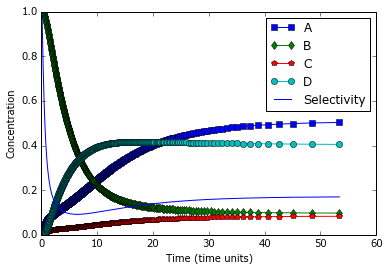
\includegraphics[max size={\textwidth}{\textheight}]{Adriaan Riet Exam_1 Problem 2_files/Adriaan Riet Exam_1 Problem 2_10_0.png}
    \par
    \end{center}
    
            \end{InvisibleVerbatim}
            
        
    


    % Make sure that atleast 4 lines are below the HR
    \needspace{4\baselineskip}

    
        \vspace{6pt}
        \makebox[0.1\linewidth]{\smaller\hfill\tt\color{nbframe-in-prompt}In\hspace{4pt}{[}4{]}:\hspace{4pt}}\\*
        \vspace{-2.65\baselineskip}
        \begin{ColorVerbatim}
            \vspace{-0.7\baselineskip}
            \begin{Verbatim}[commandchars=\\\{\}]
\PY{n}{plt}\PY{o}{.}\PY{n}{semilogy}\PY{p}{(}\PY{n}{t}\PY{p}{,}\PY{n}{dts}\PY{p}{)}
\PY{n}{plt}\PY{o}{.}\PY{n}{xlabel}\PY{p}{(}\PY{l+s}{\PYZsq{}}\PY{l+s}{Time (time units)}\PY{l+s}{\PYZsq{}}\PY{p}{)}
\PY{n}{muffle}\PY{o}{=}\PY{n}{plt}\PY{o}{.}\PY{n}{ylabel}\PY{p}{(}\PY{l+s}{\PYZsq{}}\PY{l+s}{Step Size}\PY{l+s}{\PYZsq{}}\PY{p}{)}
\end{Verbatim}

            
                \vspace{-0.2\baselineskip}
            
        \end{ColorVerbatim}
    

    

        % If the first block is an image, minipage the image.  Else
        % request a certain amount of space for the input text.
        \needspace{4\baselineskip}
        
        

            % Add document contents.
            
                \begin{InvisibleVerbatim}
                \vspace{-0.5\baselineskip}
    \begin{center}
    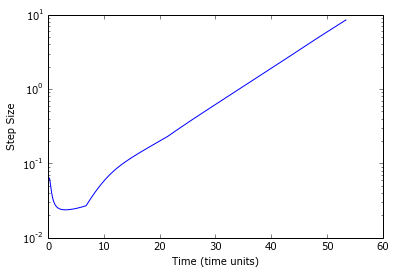
\includegraphics[max size={\textwidth}{\textheight}]{Adriaan Riet Exam_1 Problem 2_files/Adriaan Riet Exam_1 Problem 2_11_0.png}
    \par
    \end{center}
    
            \end{InvisibleVerbatim}
            
        
    
\subsection{Part b}Write a function to solve the system $Ax=b$ using the Gauss Seidel
method.

In Matlab fill in your function as:

\begin{verbatim}
function x = linear_gs(A, b)
   % write the solution here
end
\end{verbatim}

In Python, fill in your function as:

\begin{verbatim}
def linear_gs(A,b) :
    # write the solution here
    return x
\end{verbatim}

    % Make sure that atleast 4 lines are below the HR
    \needspace{4\baselineskip}

    
        \vspace{6pt}
        \makebox[0.1\linewidth]{\smaller\hfill\tt\color{nbframe-in-prompt}In\hspace{4pt}{[}5{]}:\hspace{4pt}}\\*
        \vspace{-2.65\baselineskip}
        \begin{ColorVerbatim}
            \vspace{-0.7\baselineskip}
            \begin{Verbatim}[commandchars=\\\{\}]
\PY{k+kn}{import} \PY{n+nn}{scipy.sparse}
\PY{k+kn}{from} \PY{n+nn}{scipy.sparse.linalg} \PY{k+kn}{import} \PY{n}{spsolve}
\PY{k+kn}{from} \PY{n+nn}{scipy.sparse} \PY{k+kn}{import} \PY{n}{lil\PYZus{}matrix}\PY{p}{,} \PY{n}{spdiags}
\end{Verbatim}

            
                \vspace{-0.2\baselineskip}
            
        \end{ColorVerbatim}
    


    % Make sure that atleast 4 lines are below the HR
    \needspace{4\baselineskip}

    
        \vspace{6pt}
        \makebox[0.1\linewidth]{\smaller\hfill\tt\color{nbframe-in-prompt}In\hspace{4pt}{[}6{]}:\hspace{4pt}}\\*
        \vspace{-2.65\baselineskip}
        \begin{ColorVerbatim}
            \vspace{-0.7\baselineskip}
            \begin{Verbatim}[commandchars=\\\{\}]
\PY{k}{def} \PY{n+nf}{linear\PYZus{}gs}\PY{p}{(}\PY{n}{A}\PY{p}{,}\PY{n}{b}\PY{p}{,}\PY{n}{itMax}\PY{o}{=}\PY{l+m+mi}{1000}\PY{p}{,}\PY{n}{atol}\PY{o}{=}\PY{l+m+mf}{1e\PYZhy{}6}\PY{p}{)}\PY{p}{:}
    \PY{l+s+sd}{\PYZdq{}\PYZdq{}\PYZdq{}This method requires a diagonally dominant matrix,}
\PY{l+s+sd}{    or it may diverge...\PYZdq{}\PYZdq{}\PYZdq{}}
    \PY{n}{n}\PY{p}{,}\PY{n}{m} \PY{o}{=} \PY{n}{np}\PY{o}{.}\PY{n}{shape}\PY{p}{(}\PY{n}{A}\PY{p}{)}
    \PY{n}{nb}\PY{p}{,} \PY{o}{=} \PY{n}{np}\PY{o}{.}\PY{n}{shape}\PY{p}{(}\PY{n}{b}\PY{p}{)}
    \PY{k}{if} \PY{n}{nb} \PY{o}{!=} \PY{n}{n}\PY{p}{:}
        \PY{k}{raise} \PY{n}{np}\PY{o}{.}\PY{n}{linalg}\PY{o}{.}\PY{n}{linalg}\PY{o}{.}\PY{n}{LinAlgError}\PY{p}{(}\PY{l+s}{\PYZdq{}}\PY{l+s}{A and b have different dimensions.}\PY{l+s}{\PYZdq{}}\PY{p}{)}
    \PY{n}{R} \PY{o}{=} \PY{n}{b}\PY{o}{.}\PY{n}{copy}\PY{p}{(}\PY{p}{)}
    \PY{n}{x} \PY{o}{=} \PY{n}{b}\PY{o}{.}\PY{n}{copy}\PY{p}{(}\PY{p}{)}
    \PY{n}{indx} \PY{o}{=} \PY{n}{np}\PY{o}{.}\PY{n}{arange}\PY{p}{(}\PY{l+m+mi}{0}\PY{p}{,}\PY{n}{nb}\PY{p}{)}
    \PY{n}{R}\PY{p}{[}\PY{l+m+mi}{0}\PY{p}{]}\PY{o}{=}\PY{l+m+mi}{100}
    \PY{n}{it} \PY{o}{=} \PY{l+m+mi}{0}
    \PY{n}{myBool} \PY{o}{=} \PY{n+nb+bp}{True}
    \PY{k}{while} \PY{n}{myBool}\PY{p}{:}
        \PY{n}{myBool} \PY{o}{=} \PY{n+nb+bp}{False}
        \PY{k}{for} \PY{n}{i} \PY{o+ow}{in} \PY{n+nb}{range}\PY{p}{(}\PY{n}{n}\PY{p}{)}\PY{p}{:}
            \PY{k}{if} \PY{n}{A}\PY{p}{[}\PY{n}{indx}\PY{p}{[}\PY{n}{i}\PY{p}{]}\PY{p}{,}\PY{n}{i}\PY{p}{]}\PY{o}{==}\PY{l+m+mi}{0}\PY{p}{:}
                \PY{n}{myBool} \PY{o}{=} \PY{n+nb+bp}{True}
                \PY{k}{if} \PY{n}{i} \PY{o}{==} \PY{n}{n}\PY{o}{\PYZhy{}}\PY{l+m+mi}{1}\PY{p}{:}
                    \PY{n}{i} \PY{o}{=} \PY{o}{\PYZhy{}}\PY{l+m+mi}{1}
                    \PY{k}{print}\PY{p}{(}\PY{l+s}{\PYZdq{}}\PY{l+s}{weird...}\PY{l+s}{\PYZdq{}}\PY{p}{)}
                \PY{n}{tmp} \PY{o}{=} \PY{n}{indx}\PY{p}{[}\PY{n}{i}\PY{o}{+}\PY{l+m+mi}{1}\PY{p}{]}
                \PY{n}{indx}\PY{p}{[}\PY{n}{i}\PY{p}{]}\PY{o}{=}\PY{n}{indx}\PY{p}{[}\PY{n}{i}\PY{o}{+}\PY{l+m+mi}{1}\PY{p}{]}
                \PY{n}{indx}\PY{p}{[}\PY{n}{i}\PY{o}{+}\PY{l+m+mi}{1}\PY{p}{]}\PY{o}{=}\PY{n}{tmp}
        \PY{n}{it} \PY{o}{+}\PY{o}{=}\PY{l+m+mi}{1}
        \PY{k}{if} \PY{n}{it} \PY{o}{\PYZgt{}} \PY{n}{itMax}\PY{p}{:}
            \PY{k}{print}\PY{p}{(}\PY{l+s}{\PYZdq{}}\PY{l+s}{Error, rank seems to be deficient}\PY{l+s}{\PYZdq{}}\PY{p}{)}
            \PY{k}{return} \PY{n}{b}
    \PY{n}{Err} \PY{o}{=} \PY{n}{atol}\PY{o}{*}\PY{l+m+mi}{100}
    \PY{k}{while} \PY{n}{Err}\PY{o}{\PYZgt{}} \PY{n}{atol}\PY{p}{:}
        \PY{k}{for} \PY{n}{i} \PY{o+ow}{in} \PY{n+nb}{range}\PY{p}{(}\PY{n}{n}\PY{p}{)}\PY{p}{:}
            
            \PY{n}{R}\PY{p}{[}\PY{n}{i}\PY{p}{]} \PY{o}{=} \PY{n}{b}\PY{p}{[}\PY{n}{indx}\PY{p}{[}\PY{n}{i}\PY{p}{]}\PY{p}{]}\PY{o}{.}\PY{n}{copy}\PY{p}{(}\PY{p}{)}
            \PY{k}{for} \PY{n}{j} \PY{o+ow}{in} \PY{n+nb}{range}\PY{p}{(}\PY{n}{i}\PY{p}{)}\PY{p}{:}
                \PY{n}{R}\PY{p}{[}\PY{n}{i}\PY{p}{]}\PY{o}{\PYZhy{}}\PY{o}{=} \PY{n}{A}\PY{p}{[}\PY{n}{indx}\PY{p}{[}\PY{n}{i}\PY{p}{]}\PY{p}{,}\PY{n}{j}\PY{p}{]}\PY{o}{*}\PY{n}{x}\PY{p}{[}\PY{n}{j}\PY{p}{]}
            \PY{k}{for} \PY{n}{j} \PY{o+ow}{in} \PY{n+nb}{range}\PY{p}{(}\PY{n}{i}\PY{o}{+}\PY{l+m+mi}{1}\PY{p}{,}\PY{n}{n}\PY{p}{)}\PY{p}{:}
                \PY{n}{R}\PY{p}{[}\PY{n}{i}\PY{p}{]}\PY{o}{\PYZhy{}}\PY{o}{=} \PY{n}{A}\PY{p}{[}\PY{n}{indx}\PY{p}{[}\PY{n}{i}\PY{p}{]}\PY{p}{,}\PY{n}{j}\PY{p}{]}\PY{o}{*}\PY{n}{x}\PY{p}{[}\PY{n}{j}\PY{p}{]}
            \PY{n}{x}\PY{p}{[}\PY{n}{i}\PY{p}{]} \PY{o}{=} \PY{l+m+mi}{1}\PY{o}{/}\PY{n}{A}\PY{p}{[}\PY{n}{indx}\PY{p}{[}\PY{n}{i}\PY{p}{]}\PY{p}{,}\PY{n}{i}\PY{p}{]}\PY{o}{*}\PY{n}{R}\PY{p}{[}\PY{n}{i}\PY{p}{]}
        \PY{n}{Err} \PY{o}{=} \PY{n}{np}\PY{o}{.}\PY{n}{linalg}\PY{o}{.}\PY{n}{norm}\PY{p}{(}\PY{n}{A}\PY{o}{.}\PY{n}{dot}\PY{p}{(}\PY{n}{x}\PY{p}{)}\PY{o}{\PYZhy{}}\PY{n}{b}\PY{p}{)}
        \PY{n}{it}\PY{o}{+}\PY{o}{=}\PY{l+m+mi}{1}
        \PY{k}{if} \PY{n}{it} \PY{o}{\PYZgt{}} \PY{n}{itMax}\PY{p}{:}
            \PY{k}{print}\PY{p}{(}\PY{l+s}{\PYZdq{}}\PY{l+s}{Bad day. Didn}\PY{l+s}{\PYZsq{}}\PY{l+s}{t converge. Here}\PY{l+s}{\PYZsq{}}\PY{l+s}{s my best guess.}\PY{l+s}{\PYZdq{}}\PY{p}{)}
            \PY{k}{return} \PY{n}{x}\PY{p}{[}\PY{n}{indx}\PY{p}{]}
    \PY{k}{return} \PY{n}{x}\PY{p}{[}\PY{n}{indx}\PY{p}{]}
\end{Verbatim}

            
                \vspace{-0.2\baselineskip}
            
        \end{ColorVerbatim}
    


    % Make sure that atleast 4 lines are below the HR
    \needspace{4\baselineskip}

    
        \vspace{6pt}
        \makebox[0.1\linewidth]{\smaller\hfill\tt\color{nbframe-in-prompt}In\hspace{4pt}{[}7{]}:\hspace{4pt}}\\*
        \vspace{-2.65\baselineskip}
        \begin{ColorVerbatim}
            \vspace{-0.7\baselineskip}
            \begin{Verbatim}[commandchars=\\\{\}]
\PY{n}{n} \PY{o}{=} \PY{l+m+mi}{30}
\PY{n}{D} \PY{o}{=} \PY{n}{np}\PY{o}{.}\PY{n}{array}\PY{p}{(}\PY{p}{[}\PY{n}{np}\PY{o}{.}\PY{n}{ones}\PY{p}{(}\PY{n}{n}\PY{p}{)}\PY{p}{,} \PY{o}{\PYZhy{}}\PY{l+m+mf}{1.}\PY{o}{*}\PY{n}{np}\PY{o}{.}\PY{n}{ones}\PY{p}{(}\PY{n}{n}\PY{p}{)}\PY{p}{,} \PY{l+m+mf}{4.}\PY{o}{*}\PY{n}{np}\PY{o}{.}\PY{n}{ones}\PY{p}{(}\PY{n}{n}\PY{p}{)}\PY{p}{,} \PY{o}{\PYZhy{}}\PY{l+m+mf}{1.}\PY{o}{*}\PY{n}{np}\PY{o}{.}\PY{n}{ones}\PY{p}{(}\PY{n}{n}\PY{p}{)}\PY{p}{,} \PY{n}{np}\PY{o}{.}\PY{n}{ones}\PY{p}{(}\PY{n}{n}\PY{p}{)}\PY{p}{]}\PY{p}{)}
\PY{n}{d} \PY{o}{=} \PY{p}{[}\PY{o}{\PYZhy{}}\PY{l+m+mi}{4}\PY{p}{,}\PY{o}{\PYZhy{}}\PY{l+m+mi}{2}\PY{p}{,}\PY{l+m+mi}{0}\PY{p}{,}\PY{l+m+mi}{2}\PY{p}{,}\PY{l+m+mi}{6}\PY{p}{]}
\PY{n}{A} \PY{o}{=} \PY{n}{spdiags}\PY{p}{(}\PY{n}{D}\PY{p}{,}\PY{n}{d}\PY{p}{,}\PY{n}{n}\PY{p}{,}\PY{n}{n}\PY{p}{)}
\PY{n}{b} \PY{o}{=} \PY{n}{np}\PY{o}{.}\PY{n}{random}\PY{o}{.}\PY{n}{random}\PY{p}{(}\PY{n}{n}\PY{p}{)}
\PY{n}{A} \PY{o}{=} \PY{n}{A}\PY{o}{.}\PY{n}{tocsr}\PY{p}{(}\PY{p}{)}
\PY{n}{x}\PY{o}{=}\PY{n}{linear\PYZus{}gs}\PY{p}{(}\PY{n}{A}\PY{p}{,}\PY{n}{b}\PY{p}{)}
\PY{k}{print}\PY{p}{(}\PY{n}{x}\PY{p}{)}
\end{Verbatim}

            
                \vspace{-0.2\baselineskip}
            
        \end{ColorVerbatim}
    

    

        % If the first block is an image, minipage the image.  Else
        % request a certain amount of space for the input text.
        \needspace{4\baselineskip}
        
        

            % Add document contents.
            
                \begin{InvisibleVerbatim}
                \vspace{-0.5\baselineskip}
\begin{alltt}[ 0.10318508  0.02412827  0.25020548  0.01071355  0.26521511
0.0637787
  0.23529226 -0.0110666   0.07435309  0.05489678  0.03540587
0.2848334
 -0.05205619  0.27649507  0.05317181  0.01731058  0.29727726
-0.08912096
  0.24552312  0.11171829  0.06955821  0.31652621  0.03211852
0.28580956
  0.15445159  0.04799932  0.11309191 -0.00824927  0.04557009
0.06567073]
\end{alltt}

            \end{InvisibleVerbatim}
            
        
    

        

        \renewcommand{\indexname}{Index}
        \printindex

    % End of document
    \end{document}


